%\documentclass[conference]{IEEEtran}
%\documentclass{sig-alternate}
\documentclass{sig-alternate-05-2015}

\usepackage{datatool}
%\usepackage{amsthm}
\usepackage{booktabs}
\usepackage{graphicx}
\usepackage{multirow}
\usepackage{enumerate}
\usepackage{cprotect}
\usepackage{xtab}
\usepackage{tikz}
\usepackage{url}
\usepackage{hyperref}
\usepackage{cite}
\usepackage[update,prepend,outdir=./]{epstopdf}
\DTLsetseparator{•}
\DTLloaddb{data}{../analysis_output/database.csv}

\usepackage{balance}

%submission site: http://cyberchairpro.borbala.net/asepapers/submit/
% Login: carl1978@iastate.edu
% Password: ASE-143111797041267

\widowpenalty=10000
\clubpenalty=10000

\newcommand{\todoNow}[1]{\textbf{\textcolor{red}{TODO.NOW: #1}}} %comment out for submission
\newcommand{\todoMid}[1]{\textbf{\textcolor{magenta}{TODO.MID: #1}}} %comment out for submission
%\newcommand{\todoMid}[1]{\textbf{\textcolor{magenta}{}}} %comment out for submission
\newcommand{\todoLast}[1]{\textbf{\textcolor{blue}{TODO.LAST: #1}}} %comment out for submission
\newcommand{\yes}{\tikz\draw[black,fill=black] (0,0) circle (.5ex);}
\newcommand{\sorta}{\tikz\draw[gray,fill=gray] (0,0) circle (.5ex);}
\newcommand{\no}{\tikz\draw[black] (0,0) circle (.5ex);}
\renewcommand{\dbltopfraction}{.9}
\usepackage{bigstrut}
    \setlength\bigstrutjot{2pt}
\newtheorem{mydef}{Definition}

\begin{document}
%
% paper title
% can use linebreaks \\ within to get better formatting as desired
%\title{Regex Feature Use In Practice}
%\title{Regular Expression Feature Usage in Python}
\title{Exploring  Regular Expression Usage and Context\\ in Python}

% author names and affiliations
% use a multiple column layout for up to three different
% affiliations
\numberofauthors{2}

%\author{
%\alignauthor
%Carl Chapman\\
%       \affaddr{Department of Computer Science}\\
%       \affaddr{Iowa State University}\\
%       \affaddr{Ames, IA, USA}\\
%      \email{carl1978@iastate.edu}\\
% \alignauthor
%Kathryn T. Stolee\\
%       \affaddr{Departments of Computer Science}\\
%       \affaddr{North Carolina State University}\\
%       \affaddr{Raleigh, NC, USA}\\
%      \email{ktstolee@ncsu.edu}\\
%}

% make the title area
\maketitle


\begin{abstract}
%Regular expressions are used frequently in programming languages for form validation, ad-hoc file searches, and simple parsing.
Due to the popularity and pervasive use of regular expressions, researchers have created tools to support their creation, validation, and use. However, little is known about the context in which regular expressions are used, the features that are most common, and how behaviorally similar regular expressions are to one another.
%This information is critical to inform tool designers about how to best support developers working with regular expressions.
%Each tool has made design decisions about which regular expression features to support, and these decisions impact the usefulness and power of the tools. Yet, these decisions are often made with little information as there does not exist an empirical study of regular expression feature usage to inform these design decisions.

In this paper, we explore the context in which regular expressions are used through a combination of developer surveys and repository analysis.
We survey 18 professional developers from a small software company about their regular expression usage and pain points. 
Our results indicate that developers frequently use regular expressions in their programming practices, often composing regular expressions at least weekly. 
Then, we
analyzed nearly 4,000 open source Python projects from GitHub and extracted nearly 14,000 unique regular expression patterns that were used for analysis, focusing on how often distinct features are used. 
We also map the most common features used in regular expressions to those features supported by four common regular expression engines from industry and academia: brics, Hampi, RE2, and Rex.
Using similarity analysis of regular expressions across projects,
we identify six common behavioral clusters that describe how regular expressions are often used in practice.
This is the first rigorous examination of regex usage and it provides empirical evidence to support design decisions by regex tool
builders. It also points to areas of needed future work, such as refactoring regular expressions to increase refactoring understandability, support for migrating regexes between language, and context-specific tool support for common regexes usages.   
%We conclude by discussing the implications for  tool  designers and outline several directions of future work. 
%\todoLast{Katie: revise}



%Due to the popularity and pervasive use of regular expressions, researchers have created tools to support their creation, validation, and use. However, little is known about the context in which regular expressions are used, the features that are most common, and how behaviorally similar regular expressions are to one another. This information is critical to inform tool designers about how to best support developers working with regular expressions.
%
%In this paper, we explore the context in which regular expressions are used. We survey 18 professional developers about the context and frequency of their regular expression usage. Then, we explore a sample of regular expressions, focusing on how often distinct features are used.  We analyzed nearly 4,000 open source Python projects from GitHub and extracted nearly 14,000 unique regular expression patterns that were used for analysis. We also map the most common features used in regular expressions to those features supported by four common regular expression engines from industry and academia: brics, Hampi, RE2, and Rex. Our results indicate that developers frequently use regular expressions in their programming practices, often composing regular expressions at least weekly. Using semantic analysis of regular expressions across projects, we identify six common behavioral clusters that describe how regular expressions are often used in practice. We conclude by discussing the implications for  tool  designers and outline several directions of future work.

%FYI: nProjScanned = 3898
%These observations lead to suggestions on which regular expression features are imperative to support and for future directions in research to help developers write and reuse regular expressions.
\end{abstract}

\section{Introduction }

Regular expressions (regexes) are an abstraction of keyword search that enables the identification of text using a pattern instead of an exact keyword.
Regexes are commonly used for parsing text, form validation, and text searching within text editors (e.g., emacs), command line tools (e.g., grep, sed) and IDEs (e.g., the search feature in the Eclipse IDE).  Although regexes are powerful and versatile, they can be hard to understand,  maintain, and debug, resulting in tens of thousands of bug reports~\cite{Spishak:2012:TSR:2318202.2318207}.

Due in part to their common use across programming languages and how susceptible regexes are to error, many researchers and practitioners have developed tools to support more robust creation~\cite{Spishak:2012:TSR:2318202.2318207} or to allow visual debugging~\cite{Beck:2014:RVD:2591062.2591111}. To remove the human in the loop, other research has focused on learning regular expressions from  text~\cite{Babbar:2010:CBA:1871840.1871848, Li:2008:REL:1613715.1613719}.
Beyond supporting regular expression usage, the applications of regular expressions in research include test case generation~\cite{Ghosh:2013:JAT:2486788.2486925, Galler:2014:STD:2683035.2683100, Anand:2013:OSM:2503903.2503991, Tillmann:2014:TAT:2642937.2642941},
specification for string constraint solvers~\cite{Trinh:2014:SSS:2660267.2660372, hampi}, and as queries in a data mining framework~\cite{Begel:2010:CDE:1806799.1806821} or on the semantic web~\cite{Lee:2010:PSQ:1871871.1871877}.
Regexes are also employed in critical missions like mysql injection prevention~\cite{Yeole:2011:ADT:1980022.1980229} and network intrusion detection~\cite{network}, or in more diverse applications like DNA sequencing alignment~\cite{1594922}.

These researchers and tool designers must pick what features to include or exclude, which  can be a difficult  design decision. Supporting advanced features may be more expensive, taking more time and potentially making the project too complex and cumbersome to execute well.  A selection of only the simplest of regex features limits the applicability or relevance of that work. Despite extensive research effort in the area of regex support,  no research has been done about how regexes are used in practice and what features are essential for the most common use cases.


\emph{The goal of this work is to explore 1) the context in which developers use regular expressions, and 2) the features and diversity of  regular expressions found in Python projects}.
First, we survey developers about the context of their regex usage, include how often and for what purposes regexes are composed.
Second, we measure how often regex features (e.g., kleene star, character classes, and capture groups are all features) appear in regular expressions and used in Python projects.
By comparing the features to those supported by four common regex support tools, brics~\cite{brics}, hampi~\cite{hampi}, Rex~\cite{rex}, and RE2~\cite{re2} and surveying developers about some of the less supported feature, we discuss the potential impact of omitting various features.
Third, using  a semantic analysis to cluster similar regular expressions that occur in multiple projects, we explore the most common behaviors captured by  regexes in Python.
Our results indicate that regexes are most frequently used in command line tools and IDEs, that capturing the contents of brackets and searching for delimiter characters were some of the most specific cluster behaviors, and that the capture group feature and the endpoint anchor features are the most widely used features that are poorly supported in regex tools.
The contributions of this work are:
\begin{itemize}
    \item A survey of 18 professional software developers about their experience with regular expressions,
	\item An empirical analysis of regex feature usage of nearly 14,000 regular expressions in \DTLfetch{data}{key}{nProjScanned}{value} open-source Python projects, mapping of those features to those supported by common regex tools and survey results showing the impact of not supporting various features,
	\item An approach for measuring semantic similarity of regular expressions and qualitative analysis of the most common semantically similar clusters, and
	\item A discussion of opportunities for future work in supporting programmers in writing regular expressions.
\end{itemize}

The rest of the paper is organized as follows. Section~\ref{sec:related} motivates this work by discussing research in supporting programmers in the use, creation, and validation of regular expressions. Section~\ref{sec:study} presents the research questions, survey design, and study setup for exploring regular expressions in the wild. Results of these explorations are in Section~\ref{sec:results} followed by a discussion in Section~\ref{sec:discussion}. Threats to validity are in Section~\ref{sec:threats} and the conclusion is in Section~\ref{sec:conclusion}.


\section{Related Work}
\label{sec:related}

%
%Going the other direction, a few projects have attempted to take a set of strings and generate a good regular expression that matches them like RegexGenerator++\footnote{\url{http://regex.inginf.units.it/}} and Regex-PreSuf\footnote{\url{http://search.cpan.org/~jhi/Regex-PreSuf-1.17/PreSuf.pm}} (a problem that suffers from overmatching).
%%Tools to help developers write correct regular expressions, tools like RegexBuddy, Expresso, Pythex, The Regex Coach, Regex Widget, Regex magic, RegE xr, reWork, Rubular, Txt2re and....

\todoLast{add \cite{Parnin:2013:AUJ:2589712.2589717} \cite{Callau:2011:DUD:1985441.1985448} \cite{Dyer:2014:MBA:2568225.2568295}}

Regular expressions have been a focus point in a variety of research objectives. From the user perspective, tools have been developed to support more robust creation~\cite{Spishak:2012:TSR:2318202.2318207} or to allow visual debugging~\cite{Beck:2014:RVD:2591062.2591111}.
Building on the perspective that regexes are difficult to create, other research has focused on removing the human from the creation process by learning regular expressions from  text~\cite{Babbar:2010:CBA:1871840.1871848, Li:2008:REL:1613715.1613719}.

Regarding applications, regular expressions have been used for test case generation~\cite{Ghosh:2013:JAT:2486788.2486925, Galler:2014:STD:2683035.2683100, Anand:2013:OSM:2503903.2503991, Tillmann:2014:TAT:2642937.2642941},  and
solvers for string constraints~\cite{Trinh:2014:SSS:2660267.2660372, hampi}.
Regexes are also employed in critical missions like mysql injection prevention~\cite{Yeole:2011:ADT:1980022.1980229} and network intrusion detection~\cite{network}, or in more diverse applications like DNA sequencing alignment~\cite{1594922} or querying RDF data~\cite{Lee:2010:PSQ:1871871.1871877, Alkhateeb:2009:ESR:1540656.1540975}.


As a query language, lightweight regular expressions are pervasive in search. For example,
some data mining frameworks use regular expressions as queries (e.g., ~\cite{Begel:2010:CDE:1806799.1806821}). Efforts have also been made to expedite the processing of regular expressions on large bodies of text~\cite{Baeza-Yates:1996:FTS:235809.235810}.

%One common misconception is that all regular expression languages are \emph{regular languages} which can be represented using deterministic finite automata (DFA), and so they are easy to model, easy to describe formally and execute in O(n) time.  In fact, many regular expression matching engines run in exponential time in order to support useful features such as lazy quantifiers, capturing groups, look-aheads and back-references~\cite{msdnmatching}.  In a recent regular expression library, the RE2 projext~\cite{re2}, Russ Cox aimed to use DFAs as much as possible (maximizing speed) while supporting as many useful features as possible.

%Thousands of research papers have focused on various other regular expression-related investigations.
Within standard programming languages, regular expressions libraries are very common, yet there are  differences between languages in the features that they support. For example, Java supports possessive quantifiers like \verb! `ab*+c'! (here the `+' is modifying the `*' to make it possessive) whereas Python does not.

Since  regular expression languages vary somewhat in their syntax and feature set, researchers and tool designers have typically had to pick what features to include or exclude. Thus, researchers and tool designers face a difficult design decision: supporting advanced features is always more expensive, taking more time and potentially making the tool or research project too complex and cumbersome to execute well.  A selection of only the simplest of regex features is common in research papers and automata libraries, but this limits the applicability/relevance of that work in the real world.



In this work, we perform a feature analysis on regular expressions used in the wild and compare that set to the features supported by four popular regular expression tools.
Research tools like Hampi~\cite{hampi}, and Rex~\cite{rex}, and commercial tools like brics\cite{brics} and RE2~\cite{re2}, all use regular expressions for various task. Hampi was developed  in academia and uses regular expressions as a specification language for a strong constraint solver. Rex was developed by Microsoft Research and generates strings for regular expressions that can be used in several applications, such as test case generation~\cite{Anand:2013:OSM:2503903.2503991, Tillmann:2014:TAT:2642937.2642941}. Brics is an open-source package that creates automata from regular expressions for manipulation and evaluation.
RE2 is an open-source tool created by Google to power Code Search with a more efficient regex engine.
While there are many regular expression tools available, in this work, we focus on the features support for these four tools, which offer diversity across developers (i.e., Microsoft, Google, open source, and academia) and across applications. Further, as the focus of this work is on tool designers and we wanted to perform a feature analysis, these four tools and their features are well-documented, allowing for easy comparison.

Mining properties of open source repositories is a well-studied topic, focusing, for example, on API usage patterms~\cite{Linares-Vasquez:2014:MEA:2597073.2597085} and bug characterizations~\cite{Chen:2014:ESD:2597073.2597108}.
To our knowledge, this is the first work to mine and evaluate regular expression usages from existing software repositories. Related to mining work, regular expressions have been used to form queries in mining framework~\cite{Begel:2010:CDE:1806799.1806821}, but have not been the focus of the mining activities.

% \subsection{Research on Regular Expressions}
% Visual debugging of regular expressions~\cite{Beck:2014:RVD:2591062.2591111}

% %the related work section in the Spishak section is very good re: regex tools like those that represent regexes as automata or grammars
% Static analysis to reduce errors in building regular expressions by using a type system to identify errors like {\tt PatternSyntaxExceptions} and {\tt IndexOutOfBoundsExceptions} at compile time~\cite{Spishak:2012:TSR:2318202.2318207}.

% \subsection{Research on Regular Expressions}
% Visual debugging of regular expressions~\cite{Beck:2014:RVD:2591062.2591111}

% \subsection{Research that Depends on Regular Expression Usage}
% Regular expressions are used as queries in a data mining framework~\cite{Begel:2010:CDE:1806799.1806821}



\section{Survey}
\label{sec:survey}

To understand the context of when and how programmers use regular expressions, 
we designed a survey with \todo{X} questions about regex usage. This survey was 
deployed to developers at Dwolla, a company that provides software for
 online and mobile payment management. 
 \todo{does the company want to be named in the
paper?} 
Participation was voluntary and participants were entered in a lottery for a \$50 gift card. 
The survey was completed by 20 participants. Two survey responses were excluded
because \todo{why?}, leaving 18 responses in the final data set. 



\section{Study}
\label{sec:study}

To understand how programmers use regular expressions in Python projects, we scraped \DTLfetch{data}{key}{nProjScanned}{value} Python projects from GitHub, and recorded regex usages for analysis as described in Section~\ref{study:corpus}.
Throughout the rest of this paper, we  employ the following terminology:

\noindent \textbf{Utilization}: A \emph{utilization} occurs whenever a developer uses a regex engine in a project.  We detect utilizations by recording all calls to the {\tt re} module in Python.
Within a particular file in a project, a {utilization} is composed of a function, a pattern and 0 or more flags.  Figure~\ref{fig:exampleUsage} presents an example of one regex {utilization}, with key components labeled. Specifically, {\tt re.compile} is the function call, \verb!(0|-?[1-9][0-9]*)$! is the regex string, or pattern, and {\tt re.MULTILINE} is an (optional) flag. Thought of another way, a regular expression  utilization is one single invocation of the {\tt re} library in a project.


The {utilization} in Figure~\ref{fig:exampleUsage}  will compile a regex object in the variable {\tt r1} from the pattern \verb!(0|-?[1-9][0-9]*)$!, with the \verb!$! token matching at the end of each line because of the {\tt re.MULTILINE} flag.  The pattern in this \emph{utilization} will match if it finds a zero at the end of a line, or a (possibly negative) integer at the end of a line (i.e., due to the {\tt -?} sequence denoting zero or one instance of the {\tt -}).


\begin{figure}[tb]
\centering
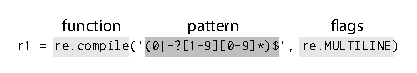
\includegraphics[width=\columnwidth]{../illustrations/exampleUsage.eps}
\caption{example of one regex utilization}
\label{fig:exampleUsage}
\end{figure}



\noindent \textbf{Pattern}: A \emph{pattern} is extracted from a utilization, as shown in Figure~\ref{fig:exampleUsage}. In essence, it is a string, but more formally it is an ordered series of regular expression language feature tokens.

Notice that because the vast majority of regex features are shared across most all-purpose languages, a Python {pattern} will (almost always) behave the same when used in other languages, such as Java, C\#, Javascript, or Ruby, whereas a utilization is not universal in the same way (i.e., it may not compile in other languages, even with small modifications to function and flag names).


% As an example, the {\tt re.MULTILINE} flag, or similar, is present in Python, Java, and C\#, but  the Python {\tt re.DOTALL} flag is not present in C\# though it has an equivalent flag in Java.
%\todo{Carl: check the above paragraph}

In this work, we primarily focus on patterns since they are cross-cutting across languages and are the primary way of specifying the matching behavior for every utilization. Next, we describe the research questions and how the data set was collected and analyzed.

\subsection{Research Questions}
\label{sec:rqs}
Our overall research goal is to understand how regular expressions and regular expression features are used in practice. We aim to answer the following research questions:

\textbf{RQ1:} How  is the {\tt re} module used in Python projects?

To address this research question, we measure how often any calls are made to the {\tt re} module per file and per project in Python projects.

Furthermore, we measure the frequency of usage for calls to the 8 functions of the {\tt re} module ({\tt re.compile}, {\tt re.search}, {\tt re.match}, {\tt re.split}, {\tt re.findall}, {\tt re.finditer}, {\tt re.sub} and {\tt re.subn}) in Python projects scraped from GitHub.

We also measure usage of the 8 flags ({\tt re.DEFAULT}, {\tt re.IGNORECASE}, {\tt re.LOCALE}, {\tt re.MULTILINE}, {\tt re.DOTALL}, {\tt re.UNICODE}, {\tt re.VERBOSE} and {\tt re.DEBUG}) of the {\tt re} module.

Further, to provide context as to the overlap among regular expression strings used in Python, we explore the most common regex {patterns} across all utlizations.

\textbf{RQ2:} Which regular expression language features are most commonly used in python?

We consider regex language features to be tokens that specify the matching behavior of a regex pattern, for example,  the {\tt +} in {\tt ab+}.  All studied features are listed and described in Section~\ref{study:corpus} with examples.

To measure feature usage, we parse Python regular expression patterns using Bart Kiers' PCRE parser\footnote{\url{https://github.com/bkiers/PCREParser}}, as described in Section~\ref{study:corpus}.  We then count the number of usages of each feature per project, per file and as a percent of all distinct regular expression patterns.

\textbf{RQ3:} What is the impact of \emph{not} supporting various regular expression features on tool designers and users?
%\textbf{RQ3:} What is the impact of \emph{not} supporting various regex features on tool designers and users?

To address, this question, we use semantic analysis to illustrate the impact of missing features on a tool's applicability by identifying what each feature (or group of features) is commonly used for.

At a high level, our semantic analysis clusters regular expressions by their behavioral similarity. Behavioral similarity is determined by a pairwise comparison among all patterns. Within each pair, a set of strings is generated for each regular expression and then tested against the other. The average percentage of matching regular expressions creates the similarity level. By calculating pairwise similarity among all regex patterns, a similarity matrix is constructed for use during clustering.

\todo{Finish this example - I will get back to this next pass}
For example, consider the following two regular expressions, denoted A and B for reference.

\begin{verbatim}
state regex A
state regex B
\end{verbatim}

For each regex, the following strings are generated:

\begin{tabular}{l | l}
A & B \\ \hline
s1 & s2 \\
s3 & s4 \\
\end{tabular}

Each string in the A column matches regex A, and each string in the B column matches regex B. When testing the strings in B against regex A, X/5 = 0.Y\% match. When testing the strings in the A column against regex B, Z/5 = 0.W\% match. Thus, the similarity between these two regular expressions is 0.U\%.

To perform this similarity analysis on each pair of regex patterns, we use Rex for string generation.  We chose Rex to build matching strings because it supports the most features of any String-generation tool. To build the similarity matrix, we generated at least 384 strings per regular expression in an effort to balance the precision of the similarity metric (i.e., more strings lead to higher precision) with the speed of our analysis tool (i.e., more strings lead to longer runtimes).

Using the similarity matrix, clusters of regexes with similar behavior are discovered using Markov Clustering\footnote{\url{http://micans.org/mcl/}}.  These clusters are used to see how programmers implement regular expressions that match similar strings and interpret what a feature is used for.
 We chose the mcl clustering tool because it offers a fast and tunable way to cluster items by similarity and it is particularly useful when the number of clusters is not known \emph{a priori}.


Next, we describe in greater detail how the corpus of regex patterns was built, how features were analyzed, and how the clustering was performed.
%\todo{Is this still the case?}
%Since our semantic analysis is based on Rex, this semantic analysis cannot be applied to all features studied.  For these unsupported features, we use 6 string similarity metrics (Jaro-Winkler, Levenshtein, Longest Common Substring, Sift3, Jaccard and Cosine) to build similarity matrices.  As before, these matrices are used to find clusters of regexes, which are used to interpret what a feature is used for.




\subsection{Building the Corpus}
\label{study:corpus}
Github is a popular project hosting site containing over 100,000 Python projects.  The GitHub API assigns an integer identifier to each repository and can be used to clone relevant repositories for analysis.  Using the \url{http://api.github.com/repositories?since=N} interface page, we launched 32 scrapers to find repositories containing Python code.  The Github interface provides information about the first 100 repository IDs since the {\tt N} value on a single results page.  Each scraper used this information to identify repositories containing Python.  When a scraper was done with one page, it continued on to the next 100 repository IDs by using the interface again with {\tt N} now equal to the last repository ID on the current page.  Using this process, each scraper paged through the next available 1,000 repositories, cloning and scanning Python projects as they were found.  Each scraper started at a different {\tt N} value, with the first scraper starting at 0.  Scraper start indices were spaced by 262,144 so as to investigate within the first 8 million repositories.  At the time scraping was performed, the highest repoID was over 32 million, so we were cloning projects in the lowest fourth of the available space of IDs.  After this process was complete, \DTLfetch{data}{key}{nProjScanned}{value} Python projects had been cloned and scanned.

For each project, we used Astroid\footnote{\url{https://bitbucket.org/logilab/astroid}} to build the AST of each Python file and find utilizations of Python's {\tt re} module. This ensured that all utliizations of the {\tt re} module were captured for analysis.

Using git, each project's commit history was scanned at 20 evenly-spaced commits.  If the project had fewer than 20 commits, then all commits were scanned.  The most recent commit was always included, and the spacing between all other chosen commits was determined by dividing the remaining number of commits by 19 (rounding as needed).

Within one project, we define a duplicate utilization as a utilization having the same function, pattern and flags within the same file (same relative path).  We ignored duplicate utilizations across project versions to protect against over-counting the same utilization as we rewind the project through its history.  We observed and recorded \DTLfetch{data}{key}{nUsages}{value} non-duplicate regex utilizations in \DTLfetch{data}{key}{nProjScanned}{value} projects.

\subsection{Extracting Patterns}
As the focus of this study is regex features, our analysis targets the patterns. Thus,  we ignore the \DTLfetch{data}{key}{percentBadFlags}{value}\%  of utilizations using flags that can alter regex behavior.  An additional \DTLfetch{data}{key}{percentInvalidPattern}{value}\% of utilizations contained patterns that could not be compiled because the pattern was non-static (e.g., used some runtime variable), or because of other unknown parsing failures.

The remaining \DTLfetch{data}{key}{percentCleanUsages}{value}\% (\DTLfetch{data}{key}{nCleanUsages}{value}) utilizations were collapsed into \DTLfetch{data}{key}{nDistinctPatterns}{value} distinct pattern strings using sql.  Each of the pattern strings was pre-processed by removing Python quotes(\verb!'\\W!' becomes \verb!\\W!), unescaping escaped characters (\verb!\\W! becomes \verb!\W!) and parsing the resulting unescaped string using an ANTLR-based, open source PCRE parser released by Bart Kiers\footnote{\url{https://github.com/bkiers/pcre-parser}}.

This parser was unable to support \DTLfetch{data}{key}{percentUnicode}{value}\% (\DTLfetch{data}{key}{N_UNICODE}{value}) of the patterns due to unsupported unicode characters.  Another \DTLfetch{data}{key}{percentAlien}{value}\% (\DTLfetch{data}{key}{N_ALIEN}{value}) of the patterns used regex features that we have chosen to exclude in this study because they did not appear often enough (e.g., Reference Conditions).  The \DTLfetch{data}{key}{nCorpus}{value} distinct pattern strings that remain were each assigned a weight value equal to the number of distinct projects the pattern appeared in.  We  refer to this set of weighted, distinct pattern strings as the \emph{corpus}.

\subsection{Analyzing Features}
\label{study:features}
For each escaped pattern, the PCRE-parser produces a tree of feature tokens. Note that features such as capture groups or logical `OR' can contain sub-patterns composed of more tokens.  For each of these trees, we counted the number of tokens, creating a frequency-of-appearance vector or `\emph{featureCount}' for each pattern.  A pattern is said to contain a feature at an index if the value of the featureCount at that index is non-zero.

\todo{fill in this paragraph for a bridge between paragraphs}
For example, consider again the pattern in Figure~\ref{fig:exampleUsage}. This pattern has X different features, specifically, Y, Z, and W. The Y feature appears X times. The set if distinct fears forms the feature set for the pattern.

Once the feature set was established, we mapped the features from the corpus to those features supported by the four regular expression engines described in Section~\ref{sec:related}: brics, hampi, RE2, and Rex.
To create the tool mappings, we consulted documentation for each of the selected regular expression engines. For brics, we collected the set of supported features using the formal grammar\footnote{\url{http://www.brics.dk/automaton/doc/index.html?dk/brics/automaton/RegExp.html}}.  For hampi, we manually inspected the set of regexes included in the {\tt lib/regex-hampi/sampleRegex} file within the hampi repository\footnote{\url{https://code.google.com/p/hampi/downloads/list}} (this may have been an overestimation, as this included more features than specified by the formal grammar\footnote{\url{http://people.csail.mit.edu/akiezun/hampi/Grammar.html}}).  For RE2, we used the  supported feature documentation\footnote{\url{https://re2.googlecode.com/hg/doc/syntax.html}}.  For Rex, we were able to use trial and error because we tried to parse all patterns with Rex, and Rex provides good error feedback when a feature is unsupported.

\todo{Were there any features supported by the tools that we did not find in the corpus? Explain either way...tomorrow.  There are many, it seems less critical}
%Our semantic analysis is dependent on the use of Rex to generate strings so we can identify semantically related clusters. For three common features unsupported by Rex, we rely on syntactic analysis to determine similarity among regular expressions containing those features. For those features supported by Rex, we cluster the regular expressions based on semantic diversity.

\subsection{Clustering and Semantic Analysis}
We are interested in what behaviors users are trying to get when using regexes, and we know that the exact same behavior, or very similar behavior can be specified in many ways.  For example, the three patterns \verb!`\W'!, \verb!`[^\w]'!, \verb!`[^a-zA-Z0-9_]'! all specify the same matching behavior.  Even if we create a slightly different pattern that matches one more character, for example \verb![\W_]!, most strings that match the first three equivalent patterns will also match the different pattern.

% \begin{figure}[tb]
% \centering
% \fbox{
% 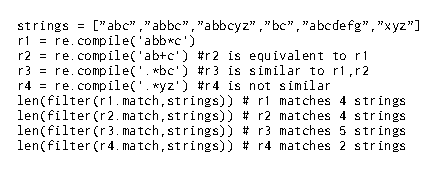
\includegraphics[width=\columnwidth]{../illustrations/equivalentPatterns.eps}
% }
% \caption{An Example of Patterns With Similar and Dissimilar Behavior}
% \label{fig:equivalentPatterns}
% \end{figure}

Rex can be used to generate a set of strings that will all match a pattern.  For each of the \DTLfetch{data}{key}{nCorpus}{value} distinct patterns, we use Rex to generate a set of at least 384 \emph{matching strings}. If fewer strings were generated, we did not include that pattern in the similarity analysis.

\todo{compute averages}
%The average number of generated strings per pattern was \todo{X} with a standard deviation of \todo{Y}. The maximum number generated was \todo{Z-these3:programming project for later tonight}.
The number 384 was selected to balance the runtime of the similarity analysis with the precision of the calculations. Since Rex does not support all the features present in the corpus, we could only generate sets of matching strings for 9,727 (70\%) of the \DTLfetch{data}{key}{nCorpus}{value} patterns in the corpus (omitted features are indicated in Table~\ref{table:featureStats} as described in Section~\ref{results:rq3}).  At least one pattern from the 9727 patterns that Rex was able to generate matching strings for can be found in 1375 of the 1645 projects containing at least one utilization.  This means that 270 projects that contained at least one utilization did not contain any Rex-compatible patterns.

As explained in Section~\ref{sec:rqs}, we used these sets of matching strings to  measure the pairwise similarity between regular expressions and create a behavioral similarity matrix.  We will refer to a cell of this matrix with row index {\tt i} and column index {\tt j} as {\tt M[i][j]}.  For each pattern at index {\tt i}, we used Rex to create a set of matching strings which we will refer to as {\tt matching\_strings\_i}.  Then for every pattern at index {\tt j}, we set the value of {\tt M[i][j]} equal to the fraction of strings in {\tt matching\_strings\_i} that the pattern at index {\tt j} matched.

Once the matrix was complete, the values of cells reflected across the diagonal of the matrix were averaged to create a half-matrix of undirected similarity edges.  Using all similarity values in this half-matrix above 0.75, we created a text file specifying the edges of a graph.  This process is illustrated in Figure~\ref{fig:matrixToGraph}.
The first matrix represents all pairwise similarity values between the four regexes: A,B,C and D.  The second matrix represents the average of cells reflected across the diagonal of the matrix.  For example the value of row A, column C (0.9) represents the similarity of C to strings generated by Rex for regex A.  The value of row C column A (0.6) represents the similarity of A to strings generated by Rex for regex C.  The average of the two values is 0.75, which goes into row C, column A in the half-matrix.  For every value of 0.75 or greater, an edge is written to \emph{out.abc}.
Note that pairs DB and DC are omitted from the graph because their similarities are lower than the threshold.  The \emph{out.abc} file generated is fed as input to the Markov Clustering Algorithm, and the top 100 clusters were catagorized by inspection into six categories of behavior.
\todo{Is the graph directed? Can you show the graph? how do the clusters emerge from the graph?}


\begin{figure}[tb]
\centering
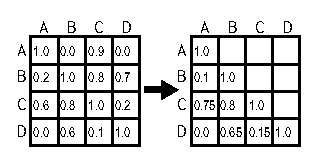
\includegraphics[width=\columnwidth]{../illustrations/matrixToGraph.eps}
\caption{Creating A Similarity Graph From A Similarity Matrix}
\label{fig:matrixToGraph}
\end{figure}
\

Markov clustering can be tuned using many parameters, including inflation and filtering out all but the top-k edges for each node.  After exploring the quality of the clusters using various tuning parameter combinations, the best clusters (by inspection) were found using an inflation value of 1.8 and k=83.

There was an operational error in pulling patterns from our database prior to the similarity analysis and clustering, so that 224 patterns (2.3\%) of the 9727 patterns that Rex was able to generate matching strings for were in fact duplicate patterns which were quoted differently (for example \verb!`\W'! and \verb!"\W"!).  The result of this error is a slight underestimate in number of projects per pattern (and per cluster), and a slight over-estimate in the pattern, file and project statistics shown in Table~\ref{table:featureStats}.  We do not believe that this error effects our conclusions.


%Most patterns do not belong in a cluster (for example a very specific pattern like \verb!<title>[^<]*Revision \d+:!), so after clustering is done only 2727 patterns are included, and only 999 projects have any of these patterns in them.



\section{Results}
\label{sec:results}



In this section, we present the results of each research question.

\subsection{RQ1: In what context do developers use regular expressions?}
\label{rq1:survey}

The survey was completed by 18 professional software developers with an average of nine years of programming experience ($\sigma = 4.28$).
On average, survey participants report to compose 172 regexes per year ($\sigma$ = 250) and compose regexes on average once per month, with 28\% composing multiple regexes in a week and an additional 22\% composing regexes once per week. That is, 50\% of respondents uses regexes at least weekly.
Table~\ref{tab:regexenviron} shows how frequently participants compose regexes using each of several languages and technical environments.
Six (33\%) of the survey participants report to compose regexes using general purpose programming languages (e.g., Java, C, C\#) 1-5 times per year and five (28\%) do this 6-10 times per year.  Regexes were rarely used in query languages like SQL, but for command line usage in tools such as grep, 6 (33\%) participants use regexes 51+ times per year.

\newcommand{\horiz}{\hspace{2.1pt}}

\begin{table}
\caption{Survey results for number of regexes composed per year by technical environment (RQ1) \label{tab:regexenviron}}
\begin{center}
\begin{small}
\begin{tabular}{l | r @{  \horiz} r @{ \horiz } r @{ \horiz } r @{ \horiz } r @{ \horiz } r }
\toprule
\textbf{Language/Environment} & 0 & 1-5 & 6-10 & 11-20 & 21-50 & 51+ \\  \hline \bigstrut
General  (e.g., Java)  & 1 & 6 & 5 & 3& 1& 2 \\ \hline \bigstrut
Scripting  (e.g., Perl) &5 &4 &3 &3 &2  &1 \\ \hline \bigstrut
Query  (e.g., SQL) & 15&2 &0 &0 &1  & 0\\ \hline \bigstrut
Command line (e.g., grep)   &2 &5 &3 &2 &0  &6 \\ \hline \bigstrut
Text editor (e.g., IntelliJ)   & 2& 5& 0& 5& 1& 5\\
\bottomrule
\end{tabular}
\end{small}
\end{center}
\end{table}

\begin{table}
\caption{Survey results for regex usage frequencies for  activities, averaged using a 6-point likert scale: Very Frequently=6, Frequently=5, Occasionally=4, Rarely=3, Very Rarely=2, and Never=1 (RQ1)\label{tab:regexactivities}}
\begin{center}
\begin{small}
\begin{tabular}{l|c}
\toprule
\textbf{Activity} & \textbf{Frequency} \\  \hline \bigstrut
Locating content within a file or files & 4.4\\ \hline \bigstrut
Capturing parts of strings & 4.3 \\ \hline \bigstrut
Parsing user input & 4.0\\ \hline \bigstrut
Counting lines that match a pattern & 3.2\\ \hline \bigstrut
Counting  substrings that match a pattern & 3.2\\  \hline \bigstrut
Parsing generated text & 3.0\\  \hline \bigstrut
Filtering collections (lists, tables, etc.) & 3.0 \\ \hline \bigstrut
Checking for a single character & 1.7\\
\bottomrule
\end{tabular}
\end{small}
\end{center}
\end{table}

Table~\ref{tab:regexactivities} shows how frequently, on average, the participants use
regexes for various actives.
Participants answered questions using a 6-point likert scale including very frequently, frequently, occasionally, rarely, very rarely, and never.
Assigning values from 1 to 6, where 6 is the most frequent, the responses were averaged across participants.
Among the most common usages are capturing parts of a string and locating content within a file, with both occurring somewhere between occasionally and frequently.

Using a similar 7-point likert scale that includes `always' as a seventh point, developers indicated that they test their regexes with the same frequency as they test their code (average response was 5.2, which is between frequently and very frequently).  Half of the 18 developers indicate that they use external tools to test their regexes, and the other half indicated that they only use tests that they write themselves. Of the nine developers using tools, six mentioned some online composition aide such as \url{regex101.com} where a regex and input string are entered, and the input string is highlighted according to what is matched.
%The other three developers mentioned 'ScalaCheck' (a testing framework), 'IDE regex plugins', and 'Language specific Regexlib'.

When asked an open ended question about pain points encountered with regular expressions, we observed three main categories. The most common, ``hard to compose," was represented in 61\% (11) responses. Next,
 39\% (7) developers responded that regexes are ``hard to read" and 17\% (3) indicated difficulties with ``inconsistency across implementations," which manifest when using regexes in multiple languages. These responses do not sum to 18 as three developers provided overlapping  answers.

\paragraph{Summary - RQ1}
%The survey validates the assumption that regex are widely used by professional software developers and sheds some light into the context in which regexes are used.
%Future research into regex can focus on activities that prove to be most important to developers, namely capturing parts of strings and searching for specific content.
%Although research into regex use in general purpose and scripting languages is important, usage within command line tools and text editors should also be considered.

Overall, regexes are used frequently with common usages including locating content within a file, capturing parts of strings, and parsing user input.
The fact that all the surveyed developers compose regexes, and half of the developers use tools to test their regexes indicates the importance of tool development for regex.  Developers complain about regex being hard to read and hard to compose, and most of the tools that they indicate using are focused on composition.



\subsection{RQ2: How  is the {\tt re} module used?}
We explore regex utilizations and flags used in the scraped Python projects.

Out of the \DTLfetch{data}{key}{nProjScanned}{value}\ projects scanned, \DTLfetch{data}{key}{percentProjectsUsingRegex}{value}\% (\DTLfetch{data}{key}{nProjectsUsingRegex}{value}) contained at least one regex utilization.  To illustrate how saturated projects are with regexes, we measure utilizations per project, files scanned per project, files contained utilizations, and  utilizations  per file, as shown in Table~\ref{table:saturation}.

The average project contained 32 utilizations, and the maximum number of utilizations was 1,427.  The project with the most utilizations is a C\# project\footnote{\url{https://github.com/Ouroboros/Arianrhod}} that maintains a collection of source code for 20 Python libraries, including larger libraries like {\tt pip}, {\tt celery} and {\tt ipython}.  These larger Python libraries contain many utilizations.
From Table~\ref{table:saturation}, we also see that each project had an average of 11 files containing any utilization, and each of these files had an average of 2 utilizations.

\begin{table}[tb]
\begin{center}
\begin{small}
\caption{How saturated are projects with utilizations? (RQ2)}
\label{table:saturation}

\begin{tabular}{l|ccccc}
\toprule
source & Q1 & Avg & Med & Q3 & Max \\ 
 \hline \bigstrut
utilizations per project & 2 & 32 & 5 & 19 & 1,427 \\ 
 \hline \bigstrut
files per project & 2 & 53 & 6 & 21 & 5,963 \\ 
 \hline \bigstrut
utilizing files per project & 1 & 11 & 2 & 6 & 541 \\ 
 \hline \bigstrut
utilizations per file & 1 & 2 & 1 & 3 & 207 \\ 
\bottomrule
\end{tabular}
\end{small}
\end{center}
\end{table}


\begin{figure}[tb]
\centering
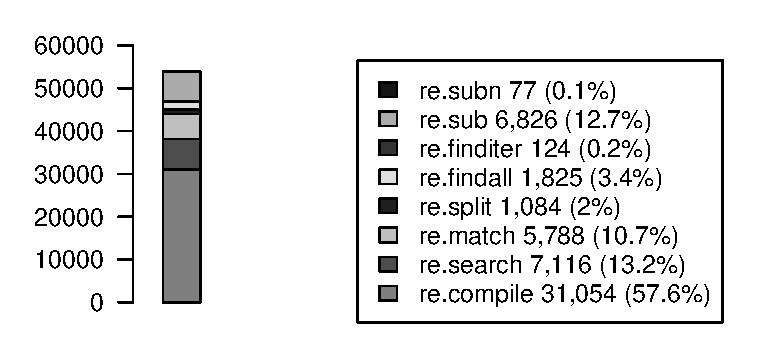
\includegraphics[width=\columnwidth]{../analysis_output/partFunctions.eps}
\vspace{-6pt}
\caption{How often are  {\tt re} functions used? (RQ2)}
\vspace{-6pt}
\label{fig:partFunctions}
\end{figure}

\begin{figure}[tb]
\centering
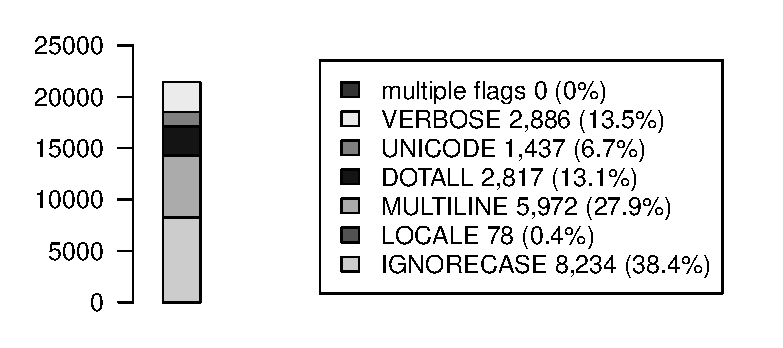
\includegraphics[width=0.9\columnwidth]{../analysis_output/partFlags.eps}
\vspace{-6pt}
\caption{Which behavioral flags are used? (RQ2)}
%\vspace{-6pt}
\label{fig:partFlags}
\end{figure}

\begin{table*}[h]
\begin{center}
\begin{small}
\caption{How Frequently do Features Appear in Projects? (RQ2)}
\label{table:featureStats}
\begin{tabular}
{ll@{ }llc@{ }c@{ }c@{ }ccccccc}
rank & code & description & example & brics & hampi & Rex & RE2 & nPatterns & \% patterns & nProjects & \% projects \\ 
\toprule[0.16em]
1 & ADD & one-or-more repetition & \begin{minipage}{0.5in}\begin{verbatim}z+\end{verbatim}\end{minipage} & \yes & \yes & \yes & \yes & 6,003 & 44.1 & 1,204 & 73.2 \\ 
\midrule
2 & CG & a capture group & \begin{minipage}{0.5in}\begin{verbatim}(caught)\end{verbatim}\end{minipage} & \yes & \yes & \yes & \yes & 7,130 & 52.4 & 1,194 & 72.6 \\ 
\midrule
3 & KLE & zero-or-more repetition & \begin{minipage}{0.5in}\begin{verbatim}.*\end{verbatim}\end{minipage} & \yes & \yes & \yes & \yes & 6,017 & 44.3 & 1,099 & 66.8 \\ 
\midrule
4 & CCC & custom character class & \begin{minipage}{0.5in}\begin{verbatim}[aeiou]\end{verbatim}\end{minipage} & \yes & \yes & \yes & \yes & 4,468 & 32.9 & 1,026 & 62.4 \\ 
\midrule
5 & ANY & any non-newline char & \begin{minipage}{0.5in}\begin{verbatim}.\end{verbatim}\end{minipage} & \yes & \yes & \yes & \yes & 4,657 & 34.3 & 1,005 & 61.1 \\ 
\midrule
6 & RNG & chars within a range & \begin{minipage}{0.5in}\begin{verbatim}[a-z]\end{verbatim}\end{minipage} & \yes & \yes & \yes & \yes & 2,631 & 19.3 & 848 & 51.6 \\ 
\midrule
7 & STR & start-of-line & \begin{minipage}{0.5in}\begin{verbatim}^\end{verbatim}\end{minipage} & \no & \yes & \yes & \yes & 3,563 & 26.2 & 846 & 51.4 \\ 
\midrule
8 & END & end-of-line & \begin{minipage}{0.5in}\begin{verbatim}$\end{verbatim}\end{minipage} & \no & \yes & \yes & \yes & 3,169 & 23.3 & 827 & 50.3 \\ 
\midrule[0.12em]
9 & NCCC & negated CCC & \begin{minipage}{0.5in}\begin{verbatim}[^qwxf]\end{verbatim}\end{minipage} & \yes & \yes & \yes & \yes & 1,935 & 14.2 & 776 & 47.2 \\ 
\midrule
10 & WSP & \textbackslash t \textbackslash n \textbackslash r \textbackslash v \textbackslash f or space & \begin{minipage}{0.5in}\begin{verbatim}\s\end{verbatim}\end{minipage} & \no & \yes & \yes & \yes & 2,846 & 20.9 & 762 & 46.3 \\ 
\midrule
11 & OR & logical or & \begin{minipage}{0.5in}\begin{verbatim}a|b\end{verbatim}\end{minipage} & \yes & \yes & \yes & \yes & 2,102 & 15.5 & 708 & 43 \\ 
\midrule
12 & DEC & any of: 0123456789 & \begin{minipage}{0.5in}\begin{verbatim}\d\end{verbatim}\end{minipage} & \no & \yes & \yes & \yes & 2,297 & 16.9 & 692 & 42.1 \\ 
\midrule
13 & WRD & [a-zA-Z0-9\_] & \begin{minipage}{0.5in}\begin{verbatim}\w\end{verbatim}\end{minipage} & \no & \yes & \yes & \yes & 1,430 & 10.5 & 650 & 39.5 \\ 
\midrule
14 & QST & zero-or-one repetition & \begin{minipage}{0.5in}\begin{verbatim}z?\end{verbatim}\end{minipage} & \yes & \yes & \yes & \yes & 1,871 & 13.8 & 645 & 39.2 \\ 
\midrule
15 & LZY & as few reps as possible & \begin{minipage}{0.5in}\begin{verbatim}z+?\end{verbatim}\end{minipage} & \no & \yes & \no & \yes & 1,300 & 9.6 & 605 & 36.8 \\ 
\midrule
16 & NCG & group without capturing & \begin{minipage}{0.5in}\begin{verbatim}a(?:b)c\end{verbatim}\end{minipage} & \no & \yes & \no & \yes & 791 & 5.8 & 404 & 24.6 \\ 
\midrule
17 & PNG & named capture group & \begin{minipage}{0.5in}\begin{verbatim}(?P<name>x)\end{verbatim}\end{minipage} & \no & \yes & \no & \yes & 915 & 6.7 & 354 & 21.5 \\ 
\midrule
18 & SNG & exactly n repetition & \begin{minipage}{0.5in}\begin{verbatim}z{8}\end{verbatim}\end{minipage} & \yes & \yes & \yes & \yes & 581 & 4.3 & 340 & 20.7 \\ 
\midrule
19 & NWSP & any non-whitespace & \begin{minipage}{0.5in}\begin{verbatim}\S\end{verbatim}\end{minipage} & \no & \yes & \yes & \yes & 484 & 3.6 & 270 & 16.4 \\ 
\midrule
20 & DBB & $n\le x \le m$ repetition & \begin{minipage}{0.5in}\begin{verbatim}z{3,8}\end{verbatim}\end{minipage} & \yes & \yes & \yes & \yes & 367 & 2.7 & 238 & 14.5 \\ 
\midrule
21 & NLKA & sequence doesn't follow  & \begin{minipage}{0.5in}\begin{verbatim}a(?!yz)\end{verbatim}\end{minipage} & \no & \no & \no & \no & 131 & 1 & 183 & 11.1 \\ 
\midrule
22 & WNW & word/non-word boundary & \begin{minipage}{0.5in}\begin{verbatim}\b\end{verbatim}\end{minipage} & \no & \no & \no & \yes & 248 & 1.8 & 166 & 10.1 \\ 
\midrule
23 & NWRD & non-word chars & \begin{minipage}{0.5in}\begin{verbatim}\W\end{verbatim}\end{minipage} & \no & \yes & \yes & \yes & 94 & 0.7 & 165 & 10 \\ 
\midrule
24 & LWB & at least n repetition & \begin{minipage}{0.5in}\begin{verbatim}z{15,}\end{verbatim}\end{minipage} & \yes & \yes & \yes & \yes & 91 & 0.7 & 158 & 9.6 \\ 
\midrule
25 & LKA & matching sequence follows & \begin{minipage}{0.5in}\begin{verbatim}a(?=bc)\end{verbatim}\end{minipage} & \no & \no & \no & \no & 112 & 0.8 & 158 & 9.6 \\ 
\midrule
26 & OPT & options wrapper & \begin{minipage}{0.5in}\begin{verbatim}(?i)CasE\end{verbatim}\end{minipage} & \no & \yes & \no & \yes & 231 & 1.7 & 154 & 9.4 \\ 
\midrule
27 & NLKB & sequence doesn't precede & \begin{minipage}{0.5in}\begin{verbatim}(?<!x)yz\end{verbatim}\end{minipage} & \no & \no & \no & \no & 94 & 0.7 & 137 & 8.3 \\ 
\midrule[0.12em]
28 & LKB & matching sequence precedes & \begin{minipage}{0.5in}\begin{verbatim}(?<=a)bc\end{verbatim}\end{minipage} & \no & \no & \no & \no & 80 & 0.6 & 120 & 7.3 \\ 
\midrule
29 & ENDZ & absolute end of string & \begin{minipage}{0.5in}\begin{verbatim}\Z\end{verbatim}\end{minipage} & \no & \no & \no & \yes & 89 & 0.7 & 90 & 5.5 \\ 
\midrule
30 & BKR & match the $i^{th}$ CG & \begin{minipage}{0.5in}\begin{verbatim}\1\end{verbatim}\end{minipage} & \no & \no & \no & \no & 60 & 0.4 & 84 & 5.1 \\ 
\midrule
31 & NDEC & any non-decimal & \begin{minipage}{0.5in}\begin{verbatim}\D\end{verbatim}\end{minipage} & \no & \yes & \yes & \yes & 36 & 0.3 & 58 & 3.5 \\ 
\midrule
32 & BKRN & references PNG & \begin{minipage}{0.5in}\begin{verbatim}\g<name>\end{verbatim}\end{minipage} & \no & \yes & \no & \no & 17 & 0.1 & 28 & 1.7 \\ 
\midrule
33 & VWSP & matches U+000B & \begin{minipage}{0.5in}\begin{verbatim}\v\end{verbatim}\end{minipage} & \no & \no & \yes & \yes & 13 & 0.1 & 15 & 0.9 \\ 
\midrule
34 & NWNW & negated WNW & \begin{minipage}{0.5in}\begin{verbatim}\B\end{verbatim}\end{minipage} & \no & \no & \no & \yes & 4 & 0 & 11 & 0.7 \\ 
\bottomrule[0.13em]
\end{tabular}
\end{small}
\end{center}
\vspace{-12pt}
\end{table*}


The number of projects that use each of the {\tt re} functions is shown in Figure~\ref{fig:partFunctions}.  The y-axis denotes the total utilizations, with a maximum of \DTLfetch{data}{key}{nUsages}{value}. The {\tt re.compile} function encompasses \DTLfetch{data}{key}{percentCompile}{value}\% of all utilizations, presumably because each usage of those functions can accept a regex object compiled using {\tt re.compile} as an argument.

When considering flag use, we excluded the default flag, which is built into the {\tt re} module, and present internally whenever no flag is used.  Of all utlizations, \DTLfetch{data}{key}{percentFlags0}{value}\% had no flag, or explicitly specified the default flag.  The debug flag, which causes the {\tt re} regex engine to display extra information about its parsing process, was never observed.
 Figure~\ref{fig:partFlags} presents the number of projects in which each flag appears. Ignorecase (\DTLfetch{data}{key}{percentI}{value}\%) and multiline (\DTLfetch{data}{key}{percentM}{value}\%) were the most frequently used.   Although multiple flags can be combined using a bitwise or, this was never observed.


\paragraph{Summary - RQ2}

Only about half of the projects sampled contained any utilizations.  Most utilizations used the {\tt re.compile} function to compile a regex object before actually using the regex to find a match.  Most utilizations did not use a flag to modify matching behavior.




%The most frequently observed patterns were used to match whitespace and digits.

\subsection{RQ3: Which regular expression language features are most commonly used in Python?}
\label{results:rq3}

To measure feature usage, we  count the number of usages of each feature per project and as a percent of all distinct regular expression patterns in the corpus.



\subsubsection{Feature Usage}
\label{sec:featureUsage}
Table~\ref{table:featureStats} displays feature usage from the corpus and relates it to four major regex related projects. Only features appearing in at least 10 projects are listed.
The first column, \emph{rank}, lists the rank of a feature (relative to other features) in terms of the number of projects in which it appears. The next column, \emph{code}, gives a succinct reference string for the feature, and is followed by a \emph{description} column that provides a brief comment on what the feature does.  The \emph{example} column provides a short example of how the feature can be used.
% For example, the most common feature observed in the corpus is \emph{one-or-more repetition}, which is specified in a pattern by using the {\tt +} character in conjunction with some sub-pattern that should repeat one or more times.  The code for this feature is \emph{ADD}, and the short example provided is \verb!z+!.
The next four columns, (i.e., \emph{brics}, \emph{hampi}, \emph{Rex}, and \emph{RE2}), map to the four major research projects chosen for our investigation (see Section~\ref{regextoolsresults}).  We indicate that a project supports a feature with the `\yes' symbol, and indicate that a project does not support the feature with the `\no' symbol.
The final four columns contain two pairs of usage statistics.  The first pair contains the number and percent of \emph{patterns} that a feature appears in, out of the 13,912 patterns that make up the corpus.  The second pair of columns contain the number and percent of \emph{projects} that a feature appears in out of the 1645 projects scanned that contain at least one utilization.

One notable omission from Table~\ref{table:featureStats} is the literal feature, which is used  to specify matching any specific character.  An example pattern that contains only one literal token is the pattern \verb!`a'!.  This pattern only matches the lowercase letter `a'.  The literal feature was found in \DTLfetch{data}{key}{P_LITERAL_PRESENT}{value}\% of patterns.
%, and accounted for \DTLfetch{data}{key}{P_LITERAL_TOKENS}{value}\% of all tokens.
We consider the literal feature to be ubiquitous in all patterns, and necessary for any regex related tool to support, and so exclude it from Table~\ref{table:featureStats} and the rest of the feature analysis.



The eight most commonly used features, ADD, CG, KLE, CCC, ANY, RNG, STR and END,
appear in over half the projects. %The remaining 26 features appear in less than half of the projects containing utilizations.
CG is more commonly used in patterns than the highest ranked feature (ADD) by a wide margin (over 8\%), even though they appear in similar numbers of projects.

\subsubsection{Feature Support in Regex Tools}
\label{regextoolsresults}
While there are many regex tools available, in this work, we focus on the features support for these four tools, brics, hampi, Rex and RE2, which offer diversity across developers (i.e., Microsoft, Google, open source, and academia) and across applications. Further, as we wanted to perform a feature analysis, these four tools and their features are well-documented, allowing for easy comparison.

% We  mapped the features from the corpus to those features supported by the four regular expression engines described in Section~\ref{sec:related}: brics, hampi, RE2, and Rex.
To create the tool mappings, we consulted documentation for each of the selected regular expression engines. For brics, we collected the set of supported features using the formal grammar\footnote{\url{http://www.brics.dk/automaton/doc/index.html?dk/brics/automaton/RegExp.html}}.  For hampi, we manually inspected the set of regexes included in the {\tt lib/regex-hampi/sampleRegex} file within the hampi repository\footnote{\url{https://code.google.com/p/hampi/downloads/list}} (this may have been an overestimation, as this included more features than specified by the formal grammar\footnote{\url{http://people.csail.mit.edu/akiezun/hampi/Grammar.html}}).  For RE2, we used the  supported feature documentation\footnote{\url{https://re2.googlecode.com/hg/doc/syntax.html}}.  For Rex, we collected the feature set empirically because we tried to parse all patterns with Rex for the semantic analysis (Section~\ref{rq4:results}), and Rex provides comprehensive error feedback for unsupported features.

%\todoLast{Were there any features supported by the tools that we did not find in the corpus? Answer: RE2 has a lot of features we didn't study and that weren't found in the corpus in any substantial quantity.  I think this is addressed by the earlier mention: Only features appearing in at least 10 projects are listed.}


Of the four projects selected for this analysis, RE2 supports the most studied features (28 features) followed by hampi (25 features),  Rex (21 features), and brics (12 features).  All projects support the 8 most commonly used features except brics, which does not support STR or END.
%All projects support NCC, OR, and the four less common repetition features: QST, SNG, DBB and LWB.  RE2 is the only project to support the WNW, ENDZ and NWNW features.
No projects support the four look-around features LKA, NLKA, LKB and NLKB.  RE2 and hampi support the LZY, NCG, PNG and OPT features, whereas brics and Rex do not.%, which inspired in part the survey questions about feature usage.


\subsubsection{Survey Results for Feature Usage}
The pattern language for Python, which is used to compose regexes, supports default character classes like the ANY or dot character class: \verb!.! meaning, `any character except newline' (a full list of features and examples is in the first four columns of Table~\ref{table:featureStats}).
It also supports three other default character classes: \verb!\d!, \verb!\w!, \verb!\s! (and their negations). All of these default character classes can be simulated using the custom character class (CCC) feature, which can create semantically equivalent regexes.
For example  the decimal character class: \verb!\d! is equivalent to a CCC containing all 10 digits:  \verb!\d! $\equiv$ \verb![0123456789]! $\equiv$ \verb![0-9]!.
%Users have a choice when using regex between writing \verb!\d! and \verb![0-9]! and whereas the first option may be shorter, the second may seem more intuitive and readable.
Other default character classes such as the word character class: \verb!\w! may not be as intuitive to encode in a CCC: \verb![a-zA-Z0-9_]!.

Survey participants were asked if they use only CCC, use CCC more than default, use both equally, use default more than CCC or use only default.  Results for this question are shown in Table~\ref{tab:cccvsdefault}, with 67\% (12) indicating that they use default the most.
Participants were also asked to explain their preferences.  Participants who favored CCC mostly said something equivalent to ``it is more explicit," whereas the participants who favored default character classes said,  ``it is less verbose" and ``I like using built-in code."

\begin{table}
\caption{Survey results for preferences between custom character and default character classes (RQ3) \label{tab:cccvsdefault}}
\begin{center}
\begin{small}
\begin{tabular}{l|c}
\toprule
\textbf{Preference} & \textbf{Frequency} \\  \hline \bigstrut
use only CCC & 1\\ \hline \bigstrut
use CCC more than default & 5 \\ \hline \bigstrut
use both equally & 2\\ \hline \bigstrut
use default more than CCC & 10\\ \hline \bigstrut
use only default & 2\\
\bottomrule
\end{tabular}
\end{small}
\end{center}
\end{table}

To further explore how frequently participants use various regex features, participants were asked five questions (on a 6-point likert scale) about how frequently they use specific related groups of features,
%\begin{itemize} \itemsep -2pt
%    \item endpoint anchors (STR, END): \verb!^! and \verb!$!
%    \item capture groups(CG): (capture me)
%    \item word boundaries (WNW): \verb!word\b!
%    \item (negative) look-ahead/behinds (LKA, NLKA, LKB, NLKB): \verb!a(?=bc)!, \verb!(?<!x)yz!, \verb!(?<=a)!, \verb!a(?!yz)!
%    \item lazy repetition (LZY): \verb!ab+?!, \verb!xy{2,3}?!
%\end{itemize}
%These features were
chosen based on the tool feature support explored in Section~\ref{regextoolsresults}.
Results are shown in Table~\ref{tab:regexfeaturegroups}, indicating that lazy repetition and look-ahead features are rarely used and capture groups and endpoint anchors are occasionally to frequently used.


\begin{table}
\caption{Survey results for regex usage frequencies, averaged using a 6-point likert scale: Very Frequently=6, Frequently=5, Occasionally=4, Rarely=3, Very Rarely=2, and Never=1 (RQ3) \label{tab:regexfeaturegroups}}
\begin{center}
\begin{small}
\begin{tabular}{llc}
\toprule
\textbf{Group} & \textbf{Code} &  \textbf{Frequency} \\  \hline \bigstrut
endpoint anchors & (STR, END) & 4.4\\ \hline \bigstrut
capture groups & (CG) & 4.2 \\ \hline \bigstrut
word boundaries & (WNW) & 3.5 \\ \hline \bigstrut
lazy repetition & (LZY) &  2.9\\ \hline \bigstrut
\multirow{2}{*}{(neg) look-ahead/behind} &  (LKA, NLKA,  & \multirow{2}{*}{2.5}\\
& LKB, NLKB) & \\
\bottomrule
\end{tabular}
\end{small}
\end{center}
\end{table}




\paragraph{Summary - RQ3}
We found that the eight most common features are found on over 50\% of the projects.
We also identify brics as the project supporting the fewest features and RE2 as the project supporting the most features, and identify groups of features supported or not supported by the four regex projects. Some of the less supported features, such as endpoint anchors and capture groups, are used by developers occasionally to frequently.
%I was confused by the 'at least occasionally' verbage, at first it looked like 'the least occasionally'

From Table~\ref{table:featureStats} we know that STR and END features are present in over half of the scanned projects containing utilizations.  In our survey, over half (56\%) of the respondents answers that they use endpoint anchors frequently or very frequently, and none of them claimed to never use them. The brics library does not support this feature, which is a missed opportunity for developers who could otherwise have used brics to model their regexes that use STR and END.

The LZY feature  is present in over 36\% of scanned projects with utilizations (Table~\ref{table:featureStats}), and yet was not supported by two of the four major regex projects we explored, brics and RE2.
In our developer survey, 11\% (2) of participants use this feature frequently and 6 (33\%) use it occasionally, showing a modest impact on potential users.

%\subsubsection{PNG and BKRN vs CG and BKR}
%The PNG group (python-style named capture groups) and BKRN (back-references: named) are intended to operate together to allow users to name the content that is expected to appear in a capture group.  A simple example of how these can be used together with the named capture group matching some vowel is:
%\verb!(?P<vowel>[aeiou]x(?P=vowel))! which will match the strings 'axa' and 'oxo' but not 'txt'.  The same functionality can be obtained with a much shorter expression: \verb!([aeiou])x\1! where the \verb!'\1'! references the CG started by the first left parenthesis found when moving from left to right.
When survey participants were asked if they prefer to always use numbered (BKR) or named (BKRN) back references, 66\% (12) of survey participants said that they always use BKR, and the remaining 33\% (6) said ``it depends."  Not one participant preferred named capture groups.  BKR is present in 5\% of scanned projects, while BKRN is present in only 1.7\%, which corroborates our findings that numbered  are generally preferred over named capture groups.

\subsection{RQ4: How behaviorally similar are regexes across projects?}
\label{rq4:results}


In clustering the regular expressions, we are interested in observing cross-project regex similarity and thus discarded patterns found in only one project.
Since Rex does not support all the regex features present in the corpus, we only generated sets of strings for measuring similarity for 2,871 (21\%) of the \DTLfetch{data}{key}{nCorpus}{value} patterns in the corpus. The impact is that 923 projects were excluded from the data set for the similarity analysis. Omitted features are indicated in Table~\ref{table:featureStats}, as described in Section~\ref{results:rq3}.
%The generated strings for each pattern are used to measure the pairwise similarity for all patterns and construct the similarity matrix.


%\subsubsection{Rationale for Behavioral Clustering}


%\subsubsection{General Information About Clusters Found}
From 2,871 distinct patterns, the MCL clustering technique identified 186 clusters with 2 or more patterns, and 2,042 clusters of size 1.  Recall that only pairs of patterns with a similarity level of 0.75 were included in the matrix passed to MCL.  The average size of clusters larger than size one was 4.5.  Each pattern belongs to exactly one cluster.

%\subsubsection{An Example Cluster}
Table~\ref{table:exampleCluster} provides an example of a behavioral cluster containing 12 patterns (4 longer patterns omitted for brevity) with at least one pattern from this cluster present in 31 different projects.  All patterns in this cluster share the literal `:' character.
%Three example strings generated by Rex for the first pattern are: `-()', `*'8(5)', `Oe()'.  For the third pattern, Rex generated these three strings: ` ()', `(q)F', `(n)M'.  The pattern: \verb!\(.*\)$! is very similar, but will not match the string `(n)M', and so was placed in a different cluster.

\begin{table}
\begin{center}
\caption{Sample from an example cluster (RQ4)}
\label{table:exampleCluster}
\begin{small}
\begin{tabular}
{lcc | lcc}
\toprule
index & pattern & nProjects & index & pattern & nProjects \\
 \hline \bigstrut
1 & \begin{minipage}{0.3in}\begin{verbatim}`:+'\end{verbatim}\end{minipage} & 8 & 5 & \begin{minipage}{0.5in}\begin{verbatim}`[:]'\end{verbatim}\end{minipage} & 6 \\
 \hline \bigstrut
2 & \begin{minipage}{0.3in}\begin{verbatim}`(:)'\end{verbatim}\end{minipage} & 8 & 6 & \begin{minipage}{0.6in}\begin{verbatim}`([^:]+):(.*)'\end{verbatim}\end{minipage} & 6 \\
 \hline \bigstrut
3 & \begin{minipage}{0.3in}\begin{verbatim}`(:+)'\end{verbatim}\end{minipage} & 8 & 7 & \begin{minipage}{0.5in}\begin{verbatim}`\s*:\s*'\end{verbatim}\end{minipage} & 4 \\
 \hline \bigstrut
4 & \begin{minipage}{0.3in}\begin{verbatim}`(:)(:*)'\end{verbatim}\end{minipage} & 8 & 8 & \begin{minipage}{0.5in}\begin{verbatim}`\:'\end{verbatim}\end{minipage} & 2 \\
\bottomrule
\end{tabular}
\vspace{-6pt}
\end{small}
\end{center}
\end{table}


%
%\begin{table}
%\begin{center}
%\caption{An example cluster (RQ3)}
%\label{table:exampleCluster}
%\begin{small}
%\begin{tabular}
%{lcc}
%\toprule
%index & pattern & nProjects\\
%\midrule
%1 & \begin{minipage}{0.5in}\begin{verbatim}`\s*,\s*'\end{verbatim}\end{minipage} & 54  \\
%\midrule
%2 & \begin{minipage}{0.5in}\begin{verbatim}`,'\end{verbatim}\end{minipage} & 30 \\
%\midrule
%3 & \begin{minipage}{0.5in}\begin{verbatim}`\s*,'\end{verbatim}\end{minipage} & 16 \\
%\midrule
%4 & \begin{minipage}{0.5in}\begin{verbatim}` ,\s*'\end{verbatim}\end{minipage} & 13 \\
%\midrule
%5 & \begin{minipage}{0.5in}\begin{verbatim}` *, *'\end{verbatim}\end{minipage} & 12 \\
%\midrule
%6 & \begin{minipage}{0.5in}\begin{verbatim}`,\S'\end{verbatim}\end{minipage} & 5 \\
%\midrule
%7 & \begin{minipage}{0.5in}\begin{verbatim}`,.*$'\end{verbatim}\end{minipage} & 3 \\
%\midrule
%8 & \begin{minipage}{0.6in}\begin{verbatim}`(\S+)\s*,\s*'\end{verbatim}\end{minipage} & 2 \\
%\midrule
%9 & \begin{minipage}{0.5in}\begin{verbatim}`,+'\end{verbatim}\end{minipage} & 1 \\
%\midrule
%10 & \begin{minipage}{0.5in}\begin{verbatim}`,\ ?'\end{verbatim}\end{minipage} & 1 \\
%\midrule
%10 & \begin{minipage}{0.5in}\begin{verbatim}`,\s*(\S)'\end{verbatim}\end{minipage} & 1 \\
%\midrule
%11 & \begin{minipage}{0.5in}\begin{verbatim}`\s*(,)\s*'\end{verbatim}\end{minipage} & 1 \\
%\midrule
%12 & \begin{minipage}{0.5in}\begin{verbatim}`\s*\,\s*'\end{verbatim}\end{minipage} & 1 \\
%\bottomrule
%\end{tabular}
%\end{small}
%\end{center}
%\end{table}


%\subsubsection{Using the Smallest Pattern to Represent a Cluster}
The smallest pattern in Table~\ref{table:exampleCluster} contains only the colon and the plus character \verb!`:+'! at index 1.  This smallest pattern gives a good idea of what all the patterns within the cluster have in common.  A shorter pattern will tend to have less extraneous behavior because it is specifying less behavior.  And yet in order for the smallest pattern to be clustered with other patterns, it had to match most of the strings created by Rex from another pattern within the cluster, and so we assume that \emph{the smallest pattern is a good representation of the cluster}.

For the rest of this paper, a cluster will be represented by one of the shortest patterns it contains, followed by the number of projects any member of the cluster appears in, so the cluster in Table~\ref{table:exampleCluster} will be represented as \verb!`:+'(31)!.

We manually mapped the top 100 largest clusters based on the number of projects into 6 behavioral categories (determined by inspection).  The largest cluster was left out, as it was composed of patterns that trivially matched almost any string, like \verb!`b*'! and \verb!`^'!.  The remaining 99 clusters were all categorized. These clusters are briefly summarized in Table~\ref{tab:clustercats}, showing the name of the category, the number of clusters it represents, number of patterns in those clusters, and the number of projects. The most common category is \emph{Multi Matches}, which contains clusters that have a disjunction of behaviors (e.g., matching a comma or semicolon, as in \verb!`,|;'(18)!). Each cluster was mapped to exactly one category. Next, we describe the categories, ordered by the number of projects the regex patterns map to.

%When a cluster can fit in multiple categories, it is placed in the most specific category.  The following six categories are listed in order from most specific behavior to least specific behavior.

\begin{table}
\begin{center}
\begin{small}
\caption{Cluster categories and sizes (RQ4) \label{tab:clustercats}}
\begin{tabular}{lccc}
\toprule
\textbf{Category} & \textbf{Clusters} & \textbf{Patterns} & \textbf{Projects} \\  \hline \bigstrut
Multi Matches & 21 & 237 & 295\\
\hline \bigstrut
Specific Char & 17 & 103 & 184\\
\hline \bigstrut
Anchored Patterns & 20 & 85 & 141\\
\hline \bigstrut
 Content of Parens & 10 & 46 & 111\\
\hline \bigstrut
Two or More Chars & 16 & 40 & 120\\
\hline \bigstrut
Code Search & 15 & 27 & 92 \\
\bottomrule
\end{tabular}
\end{small}
\end{center}
\end{table}

%6
\subsubsection{Multiple Matching Alternatives}
The patterns in these clusters match under a variety of conditions by using a character class or a disjunctive \verb!|!.
For example:
\verb!`(\W)'(89)! matches any alphanumeric character, \verb!`(\s)'(89)! matches any whitespace character, \verb!`\d'(58)! matches any numeric character, and \verb!`,|;'(18)! matches a comma or semicolon.  Most of these clusters are represented by patterns that use default character classes.  This corroborates our survey results \todoNow{this might need a n-percent of these use default cc data point, or I don't see how this is corroborating something} to the question, \emph{Do you prefer to use custom character classes or default character classes more often?}, in which 56\% (10) of the participants indicated they use the default classes more than custom.
This category contains 21 clusters, each appearing in an average of 33 projects.  These clusters have a combined total of 237 patterns, with at least one pattern present in 295 projects.

%5
\subsubsection{Specific Character Must Match}
Each cluster in this category requires one specific character to match, for example:
\verb!`\n\s*'(42)! matches only if a newline is found, \verb!`:+'(31)! matches only if a colon is found, \verb!`%'(22)!, matches only if a percent sign is found and \verb!`}'(14)! matches only if a right curly brace is found.
This behavior contrasts with the survey in Section~\ref{rq1:survey} in which participants reported to very rarely or never use regexes to check for a single character (Table~\ref{tab:regexactivities}).
This category contains 17 clusters, each appearing in an average of 17.1 projects.  These clusters have a combined total of 103 patterns, with at least one pattern present in 184 projects.

%3
\subsubsection{Anchored Patterns}
Each of the clusters uses at least one endpoint anchor to require matches to be absolutely positioned, for example:
\verb!`(\w+)$'(35)! captures the word characters at the end of the input, \verb!`^\s'(16)! matches a whitespace at the beginning of the input, and \verb!`^-?\d+$'(17)! requires that the entire input is an (optionally negative) integer.
This category contains 20 clusters, each appearing in an average of 15.4 projects.  These clusters have a combined total of 85 patterns, with at least one pattern present in 141 projects.

%2
\subsubsection{Content of Brackets and Parenthesis}
The clusters in this category center around finding a pair of characters that surround content, often also capturing that content. For example,
\verb!`\(.*\)'(29)! matches when content is surrounded by parentheses and \verb!`".*"'(25)! matches  when content is surrounded by double quotes.  The cluster \verb!`<(.+)>'(23)! matches and captures content surrounded by angled brackets.
This category contains 10 clusters, each appearing in an average of 18.4 projects.  These clusters have a combined total of 46 patterns, with at least one pattern present in 111 projects.
%, and \verb!`\[.*\]'(22)! matches when content is surrounded by square brackets
%4
\subsubsection{Two or More Characters in Sequence}
These clusters require several characters in a row to match some pattern, for example:
\verb!`\d+\.\d+'(30)! requires one or more digits followed by a period character, followed by one or more digits.  The cluster \verb!`  '(17)! requires two spaces in a row,
%\verb!`([A-Z][a-z]+[A-Z][^ ]+)'(11)!,
and \verb!`@[a-z]+'(9)! requires the at symbol followed by two or more lowercase characters, as in a twitter handle.
This category contains 16 clusters, each appearing in an average of 13 projects.  These clusters have a combined total of 40 patterns, with at least one pattern present in 120 projects.

%1
\subsubsection{Code Search and Variable Capturing}
These clusters center around a recognizable effort to parse source code or URLs and often capture variable values in it, for example:
\verb!`^https?://'(23)! matches a web address, and \verb!`(.+)=(.+)'(9)! matches an assignment statement, capturing both the variable name and value.  The cluster \\ \verb!`\$\{([\w\-]+)\}'(11)! matches an evaluated string interpolation and captures the code to evaluate.
This category contains 15 clusters, each appearing in an average of 11.7 projects.  These clusters have a combined total of 27 patterns, with at least one pattern present in 92 projects.

\paragraph{Summary - RQ4}
When tool designers are considering what features to include, data about usage in practice is valuable.  Semantic similarity clustering  helps to discern these behaviors by looking beyond the structural details of specific patterns and seeing trends in actual matching behavior.  We are also able to find out what features are being used in these behavioral trends so that we can make assertions about why certain features are important.

We used the behavior of individual patterns to form clusters, and identified six main categories that clusters belonged to.  Overall, we see that many clusters are defined by the presence of particular tokens, such as the colon for the cluster in Table~\ref{table:exampleCluster}.
These six categories define what users are doing with regexes at a high level: matching with alternatives, matching literal characters, matching with sequences, matching with endpoint anchors, parsing contents of brackets or braces, or searching and capturing Code.
One of the six common cluster categories, \emph{Code Search and Variable Capturing}, has a very specific purpose of parsing source code files. This shows a very specific and common use of regular expressions in practice.




\section{Discussion}
\label{sec:discussion}

 1111111111 PART ONE 11111111111

The results of the research questions have implications for \todo{finish me}


\emph{regex usage is usually concentrated in a few files}

Although \DTLfetch{data}{key}{percentProjectsUsingRegex}{value}\% of the projects observed had at least one regex usage, only \DTLfetch{data}{key}{percentFilesUsingRegex}{value}\% of the files observed had at least one regex usage.  This indicates that regex usage is usually concentrated in a few files.  \todo{so what?}

\noindent \emph{Observation 1: Utilizations May Be More Common In Python Library Code Than In User Code. }
The project with the most files containing utilizations: Arianrhod\footnote{\url{https://github.com/Ouroboros/Arianrhod}} which is a Japanese Anime game, mostly written in C\# (over 18K files), but containing 3404 Python files, most of which are source code for various libraries.  Of these library files, 541 (15.9\%) contain at least one utilization. \todo{so what?}


ACKk somesection about flags: notice how rarely the LOCALE flag was used.

Notice that the presence of the Verbose flag implies usage of the comment feature!



% to find the largest count for the 'utilizing files' row: select distinct uniqueSourceID, filePath, count(distinct filePath) as ct from RegexCitationMerged group by uniqueSourceID order by ct;


\subsection{DBB subsumes repetition, CCC subsumes character classes}



\todo{explain subsumption}

$a \equiv b \{0, MAX\}$

\todo{what features does DBB subsume?}

The DBB feature subsumes all other repetition features.  Consider the equivalences shown in Figure~\ref{fig:DBBequivalences}

\begin{figure}[tb]
\centering
\fbox{

\includegraphics[width=\columnwidth]{../illustrations/DBBequivalences.eps}
}
\caption{How DBB Subsumes All Other Repetition Features}
\label{fig:DBBequivalences}
\end{figure}

Similarly, the CCC feature subsumes NCCC, RNG, ANY, DEC, NDEC, WSP,NWSP, WRD, NWRD because each of these features is equivalent to a set of characters.  We provide an example of how CCC subsumes DEC, WSP and WRD in Figure~\ref{fig:CCCequivalences} (other equivalences not shown for brevity).

\begin{figure}[tb]
\centering
\fbox{

\includegraphics[width=\columnwidth]{../illustrations/CCCequivalences.eps}
}
\caption{How CCC Subsumes DEC, WSP and WRD}
\label{fig:CCCequivalences}
\end{figure}

\subsubsection{character classes are important}
In replacing keyword search with an abstracted search, one of the most fundamental abstractions is that one element of a sequence can be one of several characters.  This abstraction is realized in custom character classes.

\subsubsection{default character classes are widely used}

The pattern language for Python and most major regex engines supports a few default character classes (and their negations) which we have described as the features ANY, DEC, WSP, WRD, NDEC, NWSP, NWRD.  Throughout this analysis it was obvious that these default character classes were widely used. Specifically, \verb!\s!, \verb!\d! and \verb!\W! were the top three behavioral clusters (as shown in Table~\ref{table:topNClusters}).  In Table~\ref{table:threeClusterSample} we show the top 10 patterns from these top three clusters. \todo{implication for tool designers}


\begin{table}
\begin{center}
\caption{Top 10 Patterns in Top 3 Clusters (RQ3)}
\label{table:threeClusterSample}

\begin{tabular}
{c|c|c}
\toprule
example & example & example\\
\midrule
\begin{minipage}{0.5in}\begin{verbatim}`\s'\end{verbatim}\end{minipage} & \begin{minipage}{0.5in}\begin{verbatim}`\s'\end{verbatim}\end{minipage} & \begin{minipage}{0.5in}\begin{verbatim}`\s'\end{verbatim}\end{minipage}\\
\midrule
\begin{minipage}{0.5in}\begin{verbatim}`\s'\end{verbatim}\end{minipage} & \begin{minipage}{0.5in}\begin{verbatim}`\s'\end{verbatim}\end{minipage} & \begin{minipage}{0.5in}\begin{verbatim}`\s'\end{verbatim}\end{minipage}\\
\midrule
\begin{minipage}{0.5in}\begin{verbatim}`\s'\end{verbatim}\end{minipage} & \begin{minipage}{0.5in}\begin{verbatim}`\s'\end{verbatim}\end{minipage} & \begin{minipage}{0.5in}\begin{verbatim}`\s'\end{verbatim}\end{minipage}\\
\midrule
\begin{minipage}{0.5in}\begin{verbatim}`\s'\end{verbatim}\end{minipage} & \begin{minipage}{0.5in}\begin{verbatim}`\s'\end{verbatim}\end{minipage} & \begin{minipage}{0.5in}\begin{verbatim}`\s'\end{verbatim}\end{minipage}\\
\midrule
\begin{minipage}{0.5in}\begin{verbatim}`\s'\end{verbatim}\end{minipage} & \begin{minipage}{0.5in}\begin{verbatim}`\s'\end{verbatim}\end{minipage} & \begin{minipage}{0.5in}\begin{verbatim}`\s'\end{verbatim}\end{minipage}\\
\midrule
\begin{minipage}{0.5in}\begin{verbatim}`\s'\end{verbatim}\end{minipage} & \begin{minipage}{0.5in}\begin{verbatim}`\s'\end{verbatim}\end{minipage} & \begin{minipage}{0.5in}\begin{verbatim}`\s'\end{verbatim}\end{minipage}\\
\midrule
\begin{minipage}{0.5in}\begin{verbatim}`\s'\end{verbatim}\end{minipage} & \begin{minipage}{0.5in}\begin{verbatim}`\s'\end{verbatim}\end{minipage} & \begin{minipage}{0.5in}\begin{verbatim}`\s'\end{verbatim}\end{minipage}\\
\midrule
\begin{minipage}{0.5in}\begin{verbatim}`\s'\end{verbatim}\end{minipage} & \begin{minipage}{0.5in}\begin{verbatim}`\s'\end{verbatim}\end{minipage} & \begin{minipage}{0.5in}\begin{verbatim}`\s'\end{verbatim}\end{minipage}\\
\midrule
\begin{minipage}{0.5in}\begin{verbatim}`\s'\end{verbatim}\end{minipage} & \begin{minipage}{0.5in}\begin{verbatim}`\s'\end{verbatim}\end{minipage} & \begin{minipage}{0.5in}\begin{verbatim}`\s'\end{verbatim}\end{minipage}\\
\midrule
\begin{minipage}{0.5in}\begin{verbatim}`\s'\end{verbatim}\end{minipage} & \begin{minipage}{0.5in}\begin{verbatim}`\s'\end{verbatim}\end{minipage} & \begin{minipage}{0.5in}\begin{verbatim}`\s'\end{verbatim}\end{minipage}\\
\bottomrule
\end{tabular}
\end{center}
\end{table}



One surprising result of our clustering is that behaviorally speaking, the negation of the word class was more heavily used (208 projects) than the word class itself (114 projects).  One

The character class of all letters \verb![a-zA-Z]! appears so often that it is an excellent candidate for a new a character class.

The largest cluster using custom character classes (cluster N in Table~\ref{table:topNClusters} whose shortest member is \verb•[^ -~]•) has 44 patterns which create a more permissive word class.  Inspection of the source code of several projects using this pattern indicates that these permissive word classes were typically used when trying to create system-friendly object names, which indicates that there is a demand for a word class that includes more characters (but not dashes, tildes or the first 9 unicode characters).


22222222222222 PART TWO 22222222222

\subsection{Features That May Be Intertwined}

\todo{talk about the correlation between STR, END, noticing how their counts are nearly identical across all measures.  Yet STR seems more frequently used, suppose that with .* makes a whole line}

\todo{note that we are not comparing like projects, and that it is not a judgement on brics or something.}

\todo{Users Prefer Simple Regexes.  the top 8 features are conceptually the simplest?  Do not require thinking about steps performed by the regex engine}

\todo{What does it mean when WSP is more pervasive in patterns and files, but not projects.  That it is popular among those who are used to using it but not everyone is used to using it? Stronger correlation between nPatterns and nFiles vs nFiles and nProjects or nPatterns and nProjects}

\todo{Brics and the 6 default ccs.}


One obvious character class to consider is hexidecimal characters, and we see the pattern [a-fA-F0-9] appear many times.

For tools that do not support the default character classes, this is a significant obstacle for users trying to test the regexes that they already have.

\subsubsection{use of repetition}


\subsubsection{Anchors matter}
The endpoint anchor features STR and END are the only way specify that an entire line has to match.  Consider the following example, comparing the pattern \verb!`^\s*$'! (found in 48 projects) to the pattern \verb!`\s*'! (found in X projects) when looking for lines devoid of content.  Without the endpoint anchors, the pattern matches every line, since there are always at least zero whitespace characters on every line.  But with the endpoint anchors, only lines that contain nothing but whitespace will match, allowing the user to find all lines that don't have any content.



\subsection{Opportunities for Future Work}



\subsubsection{New library feature for properties of a line}

\subsubsection{Regexes need refactoring}
We see the same features implemented many ways, and we don't know why. It might be that some methods of implementation are more understandable. However, if tool designers do not support that, refactoring may be needed.

example with anchors and {\tt .*} in the middle which could be replaced by a comma?

\subsubsection{Using 0-9 instead of \\d}
Out of the 9727 patterns acceptable to Rex, 1498 contained the range \verb•0-9• within a character class, even though this is exactly equivalent to using \verb•\d• within a character class (which appeared within a character class only 237 times).  Why are users specifying digits using the RNG feature when a default character class already exists?  Is it to aid readability, or does this represent an opportunity for refactoring?

\subsubsection{dot-star at the end - refactoring?}
One of the most ubiquitous sub-patterns, \verb!`.*'! appeared in 1937 of the 9727 patterns acceptable by Rex, and appeared within the last four characters in 1161 of the 9727 patterns.  Out of the top 30 clusters containing the ANY feature, 26 also had \verb!`.*'! within the last four characters.

One reasonable explanation for this tendency to put \verb!`.*'! at the end of a pattern is that users want to disregard all matches after the first match on a single line in order to count how many distinct lines the match occurs on, as illustrated in Figure~\ref{fig:lineSearch}.

33333333333333 PART THREE 333333333333


\todo{NDEC is one of the most rarely used features, while DEC is one of the most frequently used default char classes.  Contrast this with the craving for NWRD behavior evident from clustering.}

\begin{figure}[tb]
\centering
\fbox{
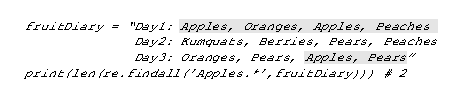
\includegraphics[width=\columnwidth]{../illustrations/lineSearch.eps}
}
\caption{An Example of Using .* to Count Lines Containing `Apples'}
\label{fig:lineSearch}
\end{figure}

In many cases, this \verb!`.*'! at the end of the string may not actually contribute any new behavior to the pattern, and may in fact be extraneous.  Or users may be trying to bypass the whole-string nature of the {\tt re.match} function, without realizing that they could instead use the {\tt re.search} function.  Consider the comparison shown in Figure~\ref{fig:searchVSmatch}

\begin{figure}[tb]
\centering
\fbox{
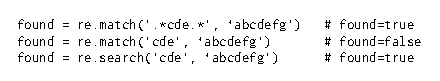
\includegraphics[width=\columnwidth]{../illustrations/matchVSsearch.eps}
}
\caption{An Example of Using .* to get Search Behavior From The Match Function}
\label{fig:searchVSmatch}
\end{figure}

Are programmers using the dot-star sub-pattern unnecessarily? More research is needed into this question to find out if these patterns are a candidate for refactoring.






Fun fact: while creating similarity matrix, row 5464 took 2 hours, or almost 1 second per cell avg, only suffering 18 timeouts (1.2 secs).  What is this pesky pattern?

We do not assume that Python projects represent a perfect sample of regular expression usage in all environments, but to make the work of collecting data for the paper reasonable, we had to choose one language to focus on (we hope to compare results across languages in future work).  Python is an attractive choice because the culture of Python programming makes it seem likely that someone would write the pattern directly in the function, not trying to over-complicate things with some extra Classes or functions.  Other attractive choices are Perl (which probably has the most active regex community), javascript and ruby (which may emphasize web tasks like form validation), sql or a general purpose language like java or C\#.




\subsection{Empirical Analysis of Regex Utilizations}


\subsection{Frequency of Feature Usage}

conclusion II

\subsubsection{A Suggested Feature Implementation Priority List}

One key consideration for Tool designers is what features are most important to implement in order of priority.  We provide a prioritized list of feature groups to implement in Figure~\ref{suggestfeaturepriority}, based on the frequency of feature usage displayed in Table~\ref{table:featureStats}.

\todo{need to list all the subsumed features for CCC and DBB. It's not clear}

\begin{figure}[tb]
\fbox{\parbox{\columnwidth}{
\begin{enumerate}
\item literals, sequences of tokens
\item CCC (and all subsumed features)
\item CG (without back-references)
\item DBB (and all subsumed features)
\item STR, END
\item OR
\item LZY
\item NCG
\item NLKA, LKA, NLKB, LKB
\item WNW, NWNW
\item ENDZ
\item BKR
\end{enumerate}
}}
\caption{A Suggested Feature Implementation Priority List \label{suggestfeaturepriority}
}
\end{figure}

\subsection{How Features Are Used In Practice}





\section{Threats to Validity}
\label{sec:threats}
The following threats impact our results and conclusions:

%\subsection{Conclusion}
\textbf{Reliability of Measures:} The validity of our survey results is dependent on the clarity of the questions. The authors went through several iterations of the survey and included examples for all the regex feature descriptions to improve understandability.

The similarity measure between regexes used in the cluster algorithm is computed empirically rather than analytically, and the more Rex-generated strings used to compute the similarity measure, the more likely it is to be accurate. Our experiments used 400 strings to balance performance and precision, but a higher number could lead to more cohesive clusters. However, regex patters that use any feature not supported by Rex were omitted from the cluster analysis. \todoMid{talk about tools for formal analysis}
%In our clustering algorithm, we require a similarity level of 0.75 so that we do not over-estimate the similarity between regular  expressions.\todoNow{what does this last sentence mean?  Is this paragraph okay?}

%\subsection{Internal}

\textbf{Instrumentation:} Regular expression patterns were clustered using strings generated by the Rex tool.  We assume that the strings generated by Rex are reasonably diverse to help characterize the regular expression behavior. To mitigate this threat, Rex generated 400 strings per regular expression and we inspected strings randomly to ensure diversity.

Implementation errors are a risk for research involving repository analysis. To combat this, we have tested our code and made the repository publicly available\footnote{\url{https://github.com/softwarekitty/tour_de_source}}.

\textbf{Selection:} We mined only \DTLfetch{data}{key}{nProjScanned}{value} Python projects from GitHub, which is  small in comparison with the over 100,000 available Python projects. The projects were mined using the GitHub API which sorts the projects by creation date. By using the API, the goal was to reduce any sampling bias introduced by the researchers.

We also did not scrape all commits in every project for regular expression utilizations, rather, we grabbed each project every 20 commits. It is possible that in between the scanned commits, a regular expression utilization was added and then removed, leading to fewer utilizations in our final data set.

\textbf{Recall bias:} The survey participants were asked to reflect on their past behavior, which may not be representative of actual behavior. To mitigate this, we designed the survey to lead the participants to think about their behavior before summarizing (e.g., asking how often they use regexes in each of several environments before asking how frequently they use regexes). 

%\subsection{Construct}

\textbf{Hypothesis guessing:} The lead author was an employee of Dwolla when the survey was run, so participant behavior may have been affected by their relationship with the author. To combat this, the beginning of the survey stated, ``As this is for research, please answer as accurately as possible, not guessing what is the desired answer and providing that."

%\subsection{External}

\textbf{Interaction of Selection and Treatment:} Our survey participants were software developers from a small startup company. However, the participants may not be representative of all developers. Given that the average participant has nine years of development experience, their responses likely pull from a variety of experiences with regular expression usage.

\textbf{Interaction of Setting and Treatment:}
We only explore regular expressions in Python projects so these results many be coupled with the activities performed using Python and not generalize to other languages. The regex usage context reported by survey participants, however, includes information on  regex usage in a  variety of settings and languages. Future work will replicate this study in other languages and the survey with a larger group of participants.



%The survey results are from a set of developers at one company and may not generalize to other developers at that company or at other companies. While the results provide some information on regex usage, repeating the survey to a larger set of diverse developers will increase the generalizeability of the results.
%%
%
%In extracting patterns for analysis, we omit utilizations that contain flags since flags provide refinements on the functionality of the pattern as it is used in the project. Given that only 12.7\% of all utilizations used flags, the impact on the clusters should be minimal.
%
%%The feature analysis is dependent on the features identified in the PCRE parser.
%



\section{Conclusion}
\label{sec:conclusion}
In this work, we have explored the contexts in which regular expressions are used as well as the features and behavioral similarities of regexes found in open source Python projects. In a survey of 18 professional developers, we find that 50\% compose regular expressions at least weekly. The most common purposes are locating content within a file or capturing parts of strings. The most difficult parts about working with regular expressions were reported to be composing and reading them.
In a study of regular expression usage in nearly 4,000 Python projects, we find that over 42\% of projects contain a regular expression.
We present an approach to measure behavioral similarity between regexes by generating strings that match one regex and pairwise  testing the remaining regexes against it. This similarity measure is used to form cross-project behavioral clusters. In the top 100 largest clusters, we find that capturing the contents of brackets,  searching for delimiter characters and matching alternative values were common behaviors.
These results have implications for tool designers and for future research aimed at better supporting developers in using regular expressions.


% use section* for acknowledgement
\section*{Acknowledgment}
Special thanks to the Dwolla developers for their survey participation.
This work is supported in part by NSF SHF-1218265, NSF SHF-EAGER-1446932, and the Harpole-Pentair endowment at Iowa State University.\\

\vspace{12pt}

\bibliographystyle{abbrv}

% The bibliography should be embedded for final submission.
\balance
\bibliography{biblio}



% that's all folks
\end{document}

